
\documentclass[11pt]{article}

\usepackage{common}
\usepackage{amsmath}
\usepackage{graphicx}

\title{HW3: (Neural) Language Modeling}
\author{Nicolas Drizard \\ nicolasdrizard@g.harvard.edu \and Virgile Audi \\ vaudi@g.harvard.edu }
\begin{document}

\maketitle{}
\section{Introduction}

This assignment focuses on the task of language modeling, a crucial first-step for many natural language applications. In this report, we will present several count-based multinomial language models with different smoothing methods, an influential neural network based language model from the work of Bengio et al. (2003), and an extension to this language model which learns using noise contrastive estimation, as well as their implementation using Torch. We found this homework more challenging than the previous ones and encountered significant challenges that we will underline in this report. 


\section{Problem Description}

The goal of the language models presented in this report is to learn a distributed representation for words as well as probability distribution for word sequences. Language models are usually represented as the probability of generating a new word conditioned on the preceeding words:

$$ P(\boldsymbol{w}_{1:n}) = \prod\limits_{i=1}^{n-1}P(w_{i+1}|w_i)$$

\noindent To simplify the analysis, it is common to make the assumption that a word is influenced only by the $N$ words immediately preceeding it, which we call the context. Even with reasonably small values for $N$, building such models are extremely expensive computationally-wise as well as time-consuming if not ran on GPU. The joint proabibility of a sequence of 6 words taken from a vocabulary of 10 000 words could possibly imply training the model to fit up to $10^{4^6}-1 =10^{24}-1$ parameters.\\

\noindent In this report, we tried implementing N-grams models in an efficient manner. Due to computational limitations (no access to GPUs...), we faced difficulties training the Neural Network and focused our efforts on building strong count-based models to solve the problem of language modeling.

% NLP is also
% full of sequences. For instance sentences, $w_1, \ldots, w_N$, where
% here $N$ is a constant length and $w_i \in \mcV$ for all
% $i \in \{1, \ldots N\}$. If we pretend sentences are all the same
% length, we can have scoring function over sentences,
% $s : \mcV^N \mapsto \reals$.  One might be defined as:

% \[ s(w_1, \ldots, w_N) = \sum_{i = 1}^N p(w_i | w_{i-2}, w_{i-1}), \]

% \noindent where $p$ is the bigram probability, which we will cover later in the class.

\section{Model and Algorithms}

Here you specify the model itself. This section should formally
describe the model used to solve the task proposed in the previous
section. This section should try to avoid introducing new vocabulary
or notation, when possible use the notation from the previous section.
Feel free to use the notation from class, but try to make the note
understandable as a standalone piece of text.

This section is also a great place to include other material that
describes the underlying structure and choices of your model, for
instance here are some example tables and algorithms from full
research papers:



\begin{itemize}
\item diagrams of your model,

  \begin{center}
    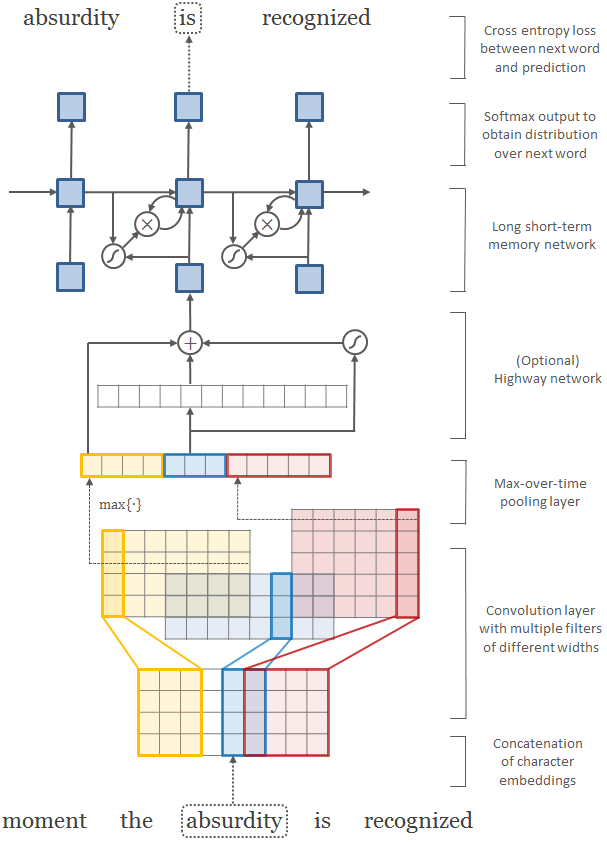
\includegraphics[width=0.4\textwidth]{network}
  \end{center}
\item feature tables,

  \begin{center}
    \begin{tabular}{@{}lll@{}}
      \toprule
      &\multicolumn{2}{c}{Mention Features  } \\
      & Feature & Value Set\\
      \midrule
      & Mention Head & $\mcV$ \\
      & Mention First Word & $\mcV$ \\
      & Mention Last Word & $\mcV$ \\
      & Word Preceding Mention & $\mcV$ \\
      & Word Following Mention & $\mcV$\\
      & \# Words in Mention & $\{1, 2, \ldots \}$ \\
      & Mention Type & $\mathcal{T}$ \\
      \bottomrule
    \end{tabular}
  \end{center}

\item pseudo-code,

  \begin{algorithmic}[1]
    \Procedure{Linearize}{$x_1\ldots x_N$, $K$, $g$}
    \State{$B_0 \gets \langle (\langle \rangle, \{1, \ldots, N\}, 0, \boldh_0, \mathbf{0})  \rangle$}
    \For{$m = 0, \ldots, M-1$ }
    \For{$k = 1, \ldots, |B_m|$}
    \For{$i \in \mcR$}
    \State{$(y, \mcR, s, \boldh) \gets \mathrm{copy}(B_m^{(k)})$}
    \For{word $w$ in phrase $x_i$}
    \State{$y \gets y $ append $w$ }
    \State{$s \gets s + \log q(w, \boldh) $ }
    \State{$\boldh \gets \delta(w, \boldh)$}
    \EndFor{}
    \State{$B_{m+|w_i|} \gets B_{m+|w_i|} + (y, \mcR - i, s,   \boldh)$}
    \State{keep top-$K$ of $B_{m+|w_i|}$ by $f(x, y) + g(\mcR)$}
    \EndFor{}
    \EndFor{}
    \EndFor{}
    \State{\Return{$B_{M}^{(k)}$}}
    \EndProcedure{}
  \end{algorithmic}

\end{itemize}


\section{Experiments}

Finally we end with the experimental section. Each assignment will make clear the main experiments and baselines that you should run. For these experiments you should present a main results table. Here we give a sample Table~\ref{tab:results}. In addition to these results you should describe in words what the table shows and the relative performance of the models.

Besides the main results we will also ask you to present other results
comparing particular aspects of the models. For instance, for word
embedding experiments, we may ask you to show a chart of the projected
word vectors. This experiment will lead to something like
Figure~\ref{fig:clusters}. This should also be described within the
body of the text itself.


\begin{table}[h]
\centering
\begin{tabular}{llr}
 \toprule
 Model &  & Acc. \\
 \midrule
 \textsc{Baseline 1} & & 0.45\\
 \textsc{Baseline 2} & & 2.59 \\
 \textsc{Model 1} & & 10.59  \\
 \textsc{Model 2} & &13.42 \\
 \textsc{Model 3} & & 7.49\\
 \bottomrule
\end{tabular}
\caption{\label{tab:results} Table with the main results.}
\end{table}


\begin{figure}
  \centering
  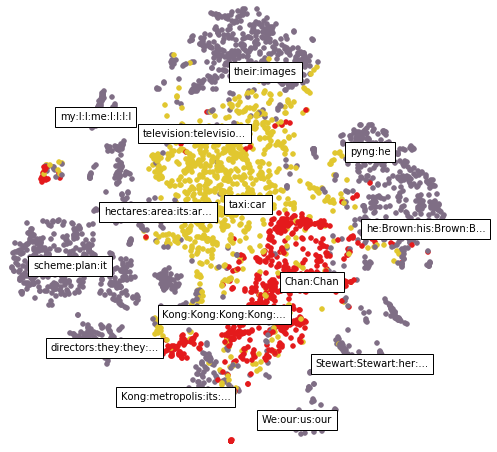
\includegraphics[width=6cm]{cluster_viz}
  \caption{\label{fig:clusters} Sample qualitative chart.}
\end{figure}


\section{Conclusion}

End the write-up with a very short recap of the main experiments and the main results. Describe any challenges you may have faced, and what could have been improved in the model.

\bibliographystyle{apalike}
\bibliography{writeup}

\end{document}
